\chapter{Evaluation}

\begin{chapterintro}

In this chapter we will analyse the behaviour and performance of the system. We will also evaluate the accuracy of its responses, and the end user experience compared to a regular \ac{QA} system.
 
\end{chapterintro}

\cleardoublepage

\section{Overview}

The systems developed for this project has multiple modules of systems, each one of them with different hardware requirements. Therefore, we will first take a look at the performance for each module, to then focus in measuring the response of the entire system.

Together with the performance analysis, we have run a experiment to analyse the effect on the end user experience of the system, compared to a regular \ac{QA} system, using the Java prototype. To do so, we implemented a simple \ac{QA} and then presented a reduced group of users with both systems, asking them to evaluate both systems.

\section{Requirements and Benchmark}

For our system, we will first analyse the memory and CPU usage under low load for each of the modules. The results can be seen in table \ref{tab:loadmeasures}.

\emph{\textcolor{red}{Update with values from munin, and graphs}}
  
\begin{table}
  \centering
  \begin{tabular*}{0.7\textwidth}{| c | c | c |}
    \hhline{|-|-|-|}
    \textbf{Module} & \textbf{CPU Usage} & \textbf{Memory} \\ \hhline{|=|=|=|}
    ChatScript & 0.2 \% &  140MB \\ \hhline{|-|-|-|}
    Solr & 1.9 \% & 533.74MB \\ \hhline{|-|-|-|}
    Python Controller & 0.2 \% & 12.66MB \\ \hhline{|-|-|-|} 
    \end{tabular*}
  \caption{Memory and CPU usage for each system under low load}
  \label{tab:loadmeasures}
\end{table}

This measures where performed on a system running Debian Jessie, with the components shown in table \ref{tab:systeminfo}

\emph{\textcolor{red}{Check memory and hard drive vendor}}
\begin{table}
  \centering
  \begin{tabular*}{0.5\textwidth}{| c | c |}
    \hhline{|-|-|}
    Motherboard & Asus V-P7H55E \\ \hhline{|-|-|} 
    CPU & Intel i5 650 3.20GHz  \\ \hhline{|-|-|} 
    Memory & Dual Channel 4096MB  \\ \hhline{|-|-|} 
    Hard Drive & \\ \hhline{|-|-|} 
    \end{tabular*}
  \caption{Memory and CPU usage for each system under low load}
  \label{tab:systeminfo}
\end{table}


Figures \ref{fig:cpuuse} and \ref{fig:memuse} show CPU and memory usage for the controller and ChatScript over time.


\begin{figure}[!htbp]
    \centering
    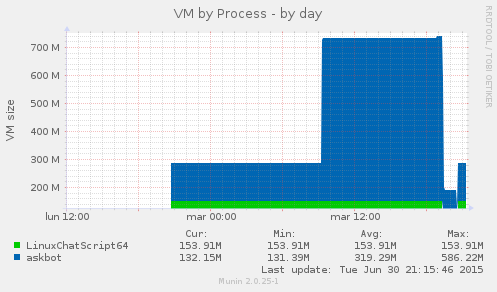
\includegraphics[width=0.7\textwidth]{img/test/memory_by_process.png}
    \caption{Memory consumption from ChatScript and the controller}
    \label{fig:memuse}
\end{figure}


\begin{figure}[!htbp]
    \centering
    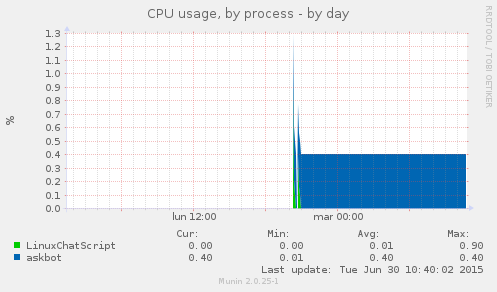
\includegraphics[width=0.7\textwidth]{img/test/cpu_usage.png}
    \caption{CPU usage for ChatScript and the controller}
    \label{fig:cpuuse}
\end{figure}

We have also attempted to measure the response time for the system for a number of different queries for a remote system. Figure \ref{fig:times-demos} shows the measured times.

\begin{figure}[!htbp]
    \centering
    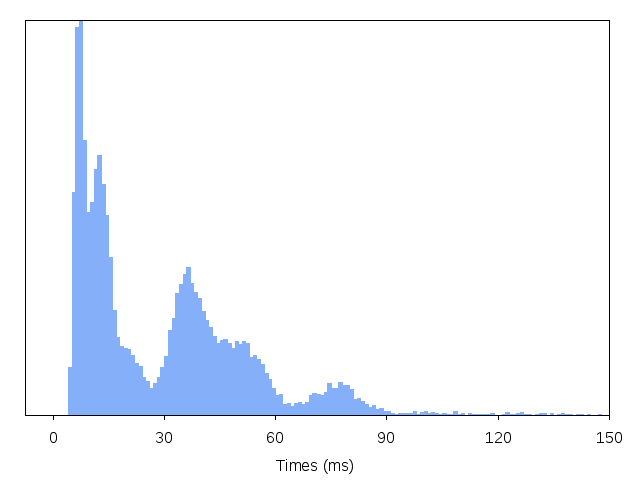
\includegraphics[width=0.8\textwidth]{img/test/times.png}
    \caption{Times for queries}
    \label{fig:times-demos}
\end{figure}

\section{Corpus tests}

During the development of the system, we prepared a corpus, to be able to test it in an automated way.

\section{User experience}

Finally, we tested the system in a trial with users, comparing the Java prototype to a regular \ac{QA} system. The users are presented both interfaces, shown in figures \ref{fig:qa-client-for} and \ref{fig:ask-client-for}, with a similar aspect to prevent the effect of different interfaces to have an effect in the results. The \ac{QA} will search for the information in the indexed documents, and show the result in the screen, whereas our system will behave as described in chapter \ref{chap:usecasejava}

The participants of the experiment ranged in age from 20 to 30 years old, most of them being under 25. 15\% of them where female, and 69\% of them where students. All of them had indicated they had experience with computers, and knowledge of the Java programming language, but none of them had participated in any previous study involving conversational agents.

\begin{figure}[!htbp]
    \centering
    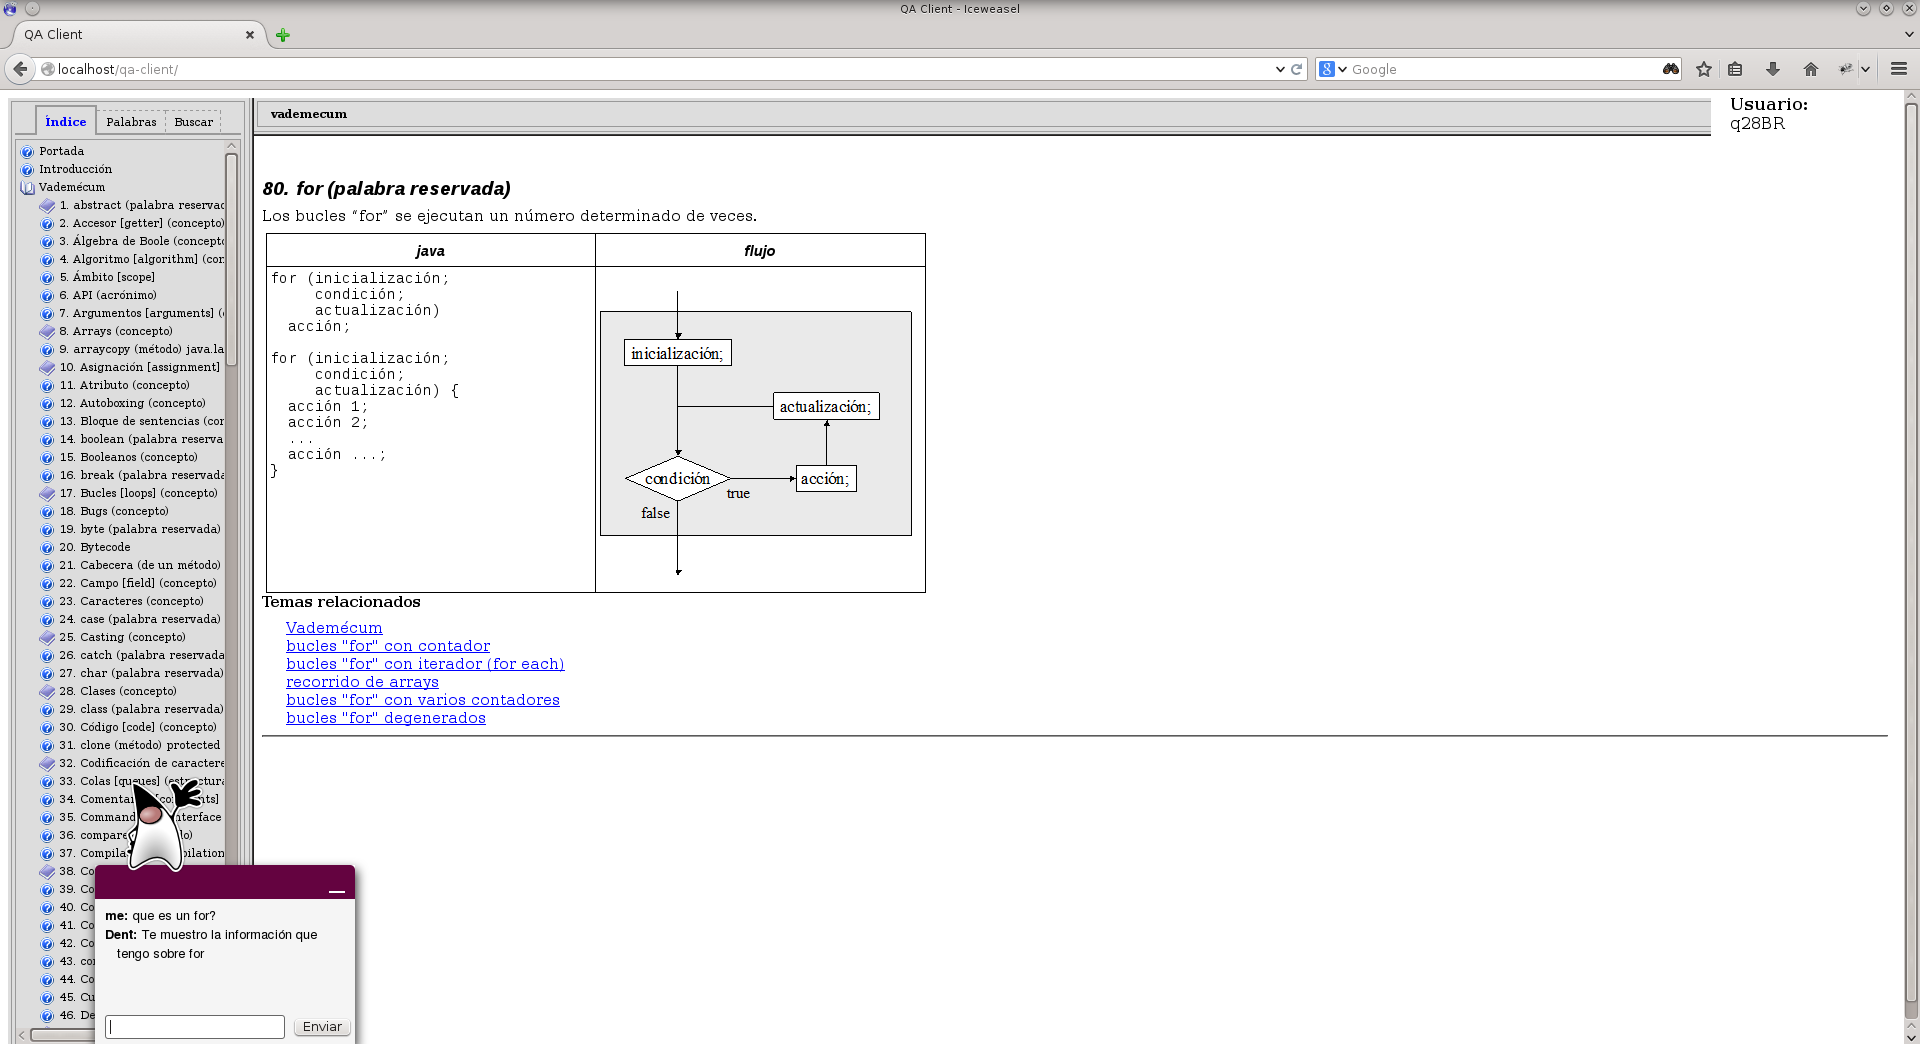
\includegraphics[width=0.7\textwidth]{img/test/qa-client2.png}
    \caption{QA interface after asking about the for loop}
    \label{fig:qa-client-for}
\end{figure}

\begin{figure}[!htbp]
    \centering
    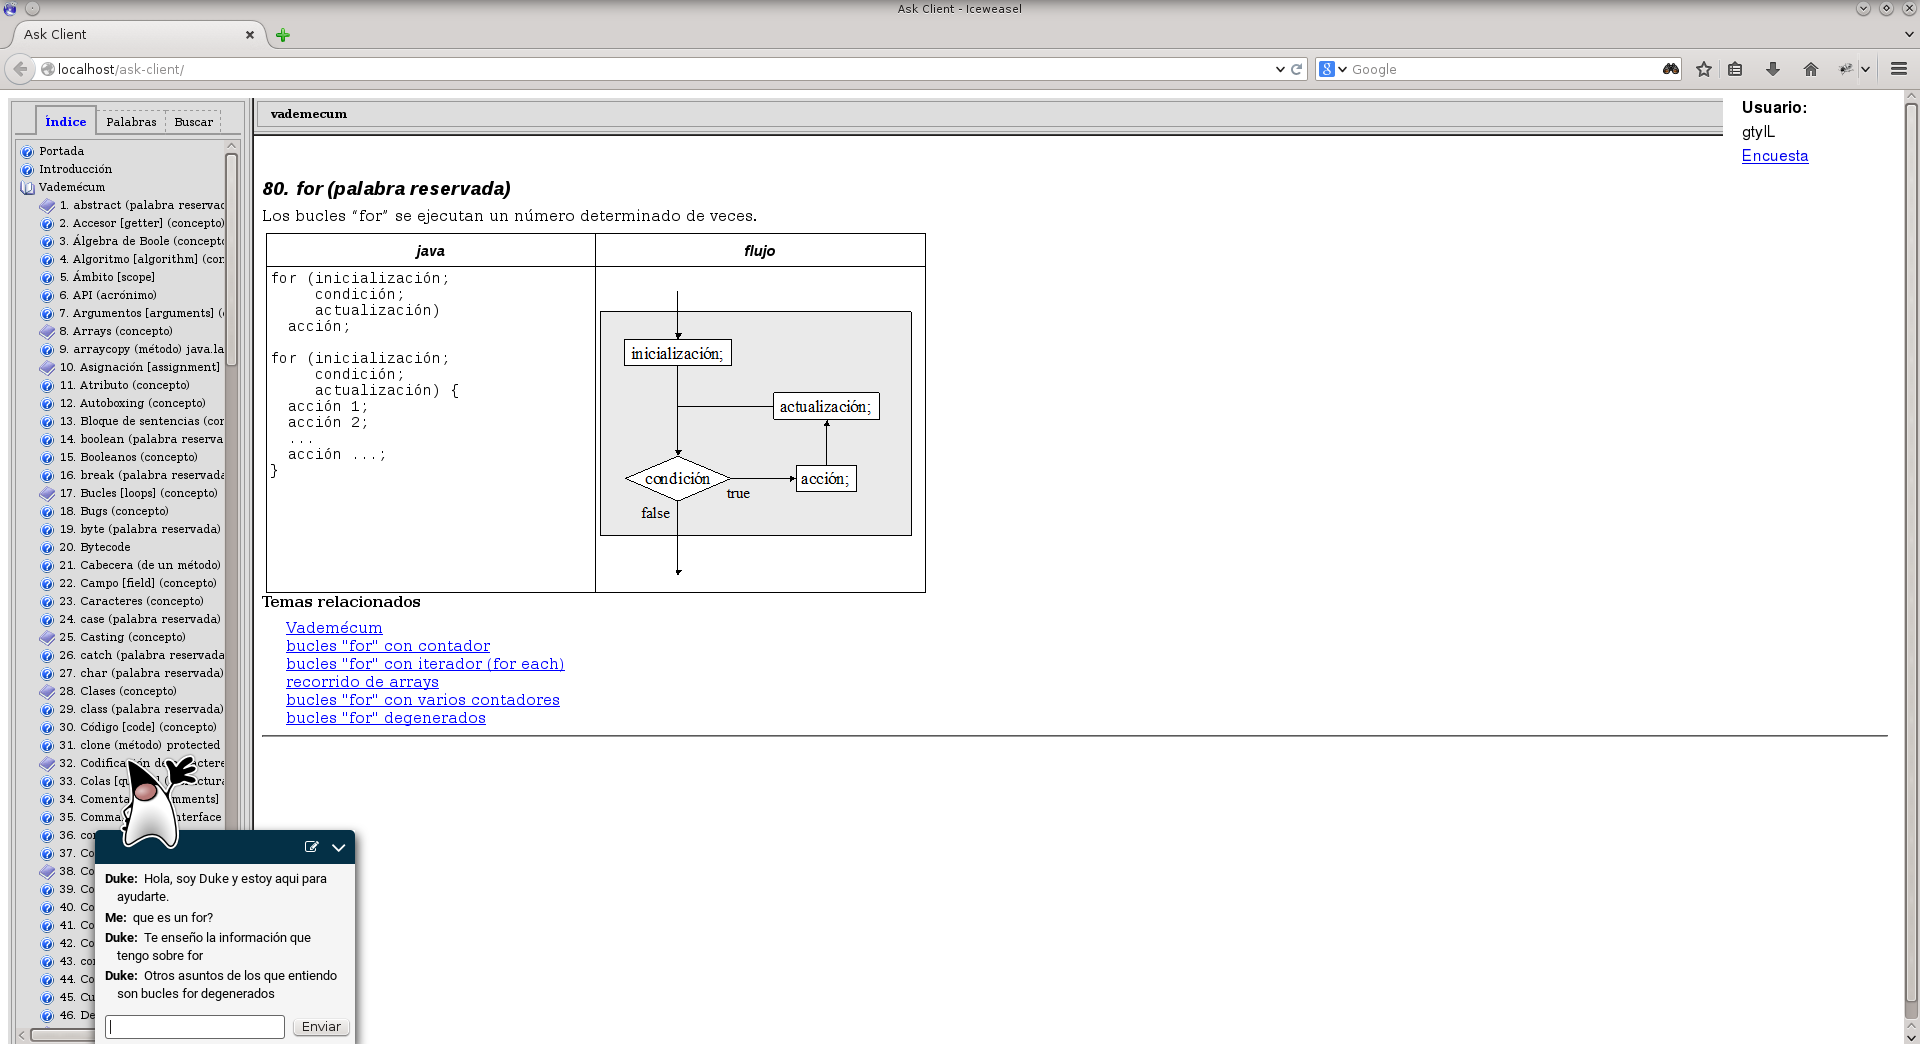
\includegraphics[width=0.7\textwidth]{img/test/ask-client.png}
    \caption{Interface for our system about the for loop}
    \label{fig:ask-client-for}
\end{figure}

\emph{\textcolor{red}{Check this sections}}

\subsection{Experiment procedure}


We proposed the participants to interact with two different configurations of our prototype. They are presented a \ac{QA} configuration and a Conversational Agent configuration (both with similar interfaces in order to avoid the effect of the possible confounding variable). The \ac{QA} search for the information in the documents available and shows the result. Indeed, with this configuration, the \ac{QA} system is working as a \ac{IR} since it does not extract any information from the document. This is simple but yet valid and useful configuration since the documents we worked with were relatively small. The second configuration consist on a conversational agent, that have access to the same information as the former system (and uses the same \ac{IR} module), with the added features of social dialog and proactive recommendation of related topic and suggesting examples. In both cases, some answers will be served with suggestions of related topics and examples to ask for. Instead of implementing four different configurations of the system, this approach was selected because the influence of the suggestions can still be measured, and otherwise the learning and fatigue effects of within-subjects evaluation with too many interfaces (that are very similar) may falsify the results.


We hypothesise that participants will prefer using natural language rather than keywords search to query the system, and that they will mostly follow the suggestions given, specially in the Conversational Agent configuration. Particularly we state the following hypothesis:

\begin{itemize}
  \item \textbf{Hypothesis 1:} Participants will interact more times with the conversational agent interface than with the QA interface.    
  \item \textbf{Hypothesis 2a:} Participants will use natural language queries significantly more times than keyword queries to consult the system.
  \item \textbf{Hypothesis 2b:} In particular, participants will use natural language queries slightly more times with the conversational agent interface than with the QA interface.
  \item \textbf{Hypothesis 3a:} Participants will prefer to follow suggestions and ask for related topics significantly more times rather than asking for different topics.
  \item \textbf{Hypothesis 3b:} In particular, participants will prefer to follow suggestions when these are offered so that they have to accept or reject them.
% \item Hypothesis 3: Participants will interact significantly more times with the Conversational Agent system than with the Question Answering system. 
%   \item \textbf{Hypothesis 4a:} Participants who engage in social dialogue will interact significantly more times than those who do not.
  \item \textbf{Hypothesis 4:} Participants who engage in social dialogue will show significantly more satisfaction in the questionnaire.  
\end{itemize}


The 12 participants that volunteered for this evaluation process were randomly assigned to one of two groups, varying the order in which they will evaluate the two interfaces for counterbalancing (50\% of the participants will test the QA configuration first and then the Conversational Agent). Each group receives a evaluation guide and a questionnaire. Each participant is given the task consisting on questioning the system (to add extra motivation we encouraged them to try to trick it or find a relevant topic where to which the system has no answer). They are requested to perform this task with both system configuration.
The evaluation consist on: first, the participants fill in a demographics questionnaire; second, they are given the general instructions to follow in the whole evaluation process; then they are given the task and the url of the system they will test first (according to the group the belong to); after that, they are requested to fill in a questionnaire of satisfaction about the first system configuration; then they are given the url of the second system to test (and the same task to perform); a second satisfaction questionnaire about the second system configuration is delivered; and finally they are requested to fill in a global satisfaction questionnaire. The average time for performing the whole evaluation process was 9.13 minutes (SD=4.26).



\subsection{Measurements}

During the process, two different measurements were taken: the questionnaires of satisfaction delivered three times during the process, and the interaction measurements taken from the logs resulting from the interaction of each participant with the system. The questionnaires and the interaction measurements were paired using unique session identifiers. After the evaluation process the logs were computed to obtain five metrics: the number of total interactions of each participant with each system configuration, the number of suggestions received by each participant with each configuration, the number of suggestions followed by each participant with each configuration, the format of each participant's query (Natural language or keywords) with each configuration, and the number of participants that interacted using social dialog with each configuration.

\subsubsection{Usage of different type of queries}

We split the user queries into two groups: those formed \ac{NL} and those that basically formed of keywords. Although in different measure 75\% of the participants used a keyword query at least once, and all of them used \ac{NL} queries. The average number of \ac{NL} queries per use was 6.79, 1.26 times greater than the average number of keyword-based queries. It is statistically significant (F\textsubscript{1,11}=9.82, p=0.004~\textless~.005) that prefer \ac{NL} to consult rather than keyword-based queries. This is also verifiable when we split the data of both interfaces. Resulting p values are 0.011 and 0.008 for \ac{QA} and conversational agent configurations respectively. This support out hypothesis 2a.
% 
However, it is not statistically significant that users use more often \ac{NL} than keywords with the Conversational Agent than with the QA configuration, so hypothesis 2b cannot be validated. Figure~\ref{fig:exp_querytype} shows this distribution, and it can be appreciated that the number of interactions increases with the Conversational Agent configuration for both query types.
We concluded this is because, users in general have their own preferences about use natural language or keywords (or possibly influenced by the nature of the interface used) regardless of the nature of the answers received.
It is important to point out that only two out of 12 users in the experiment used more often keyword queries than \ac{NL} queries
Here there exists a subtle group effect, since users from Group B (which interacted first with the conversational agent) slightly reduced the usage of Keyword queries when they interacted with the \ac{QA} interface.

\begin{figure}[!tbh]
  \centering
  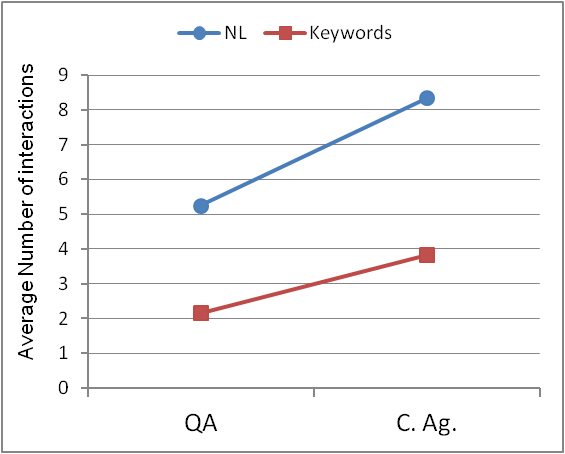
\includegraphics[width=0.8\textwidth]{img/test/exp_querytype.png}
  \DeclareGraphicsExtensions.  
  \caption{Average number of interactions per user using each query type for each system configuration}
  \label{fig:exp_querytype}
\end{figure}

\subsubsection{Impact of suggestions}

An average of 57\% of the times a user was given a suggestion he/she followed that suggestion in the next interaction. Besides, users rated the usefulness of suggestions with 3.41 over 4. However, 96\% of the suggestions followed were close-ended questions, e.g. ``Do you want to check for {\em inheritance} too?''. Thus we can conclude that users are interested in suggestions when they only need to accept or reject them (hypothesis 3b), but not that they follow suggestions of any type (hypothesis 3a). In out experiment, we decide to give suggestions in pairs (e.g. ``you may me interested in searching for topic A or topic B'') and it may be not the best approach to persuade the user to follow them.
% Or maybe they did not take the tool seriously, so they simply asked purposeless.


\subsubsection{Satisfaction}

According to the results shown in Fig.~\ref{fig:exp_satisfaction}, no correlation between interaction metrics and user's satisfaction is appreciated. Thus we cannot validate hypothesis 4. 
% We concluded that we need to take into account second or third degree metrics and also increase the number of participants.

\begin{figure}[!tbh]
  \centering
  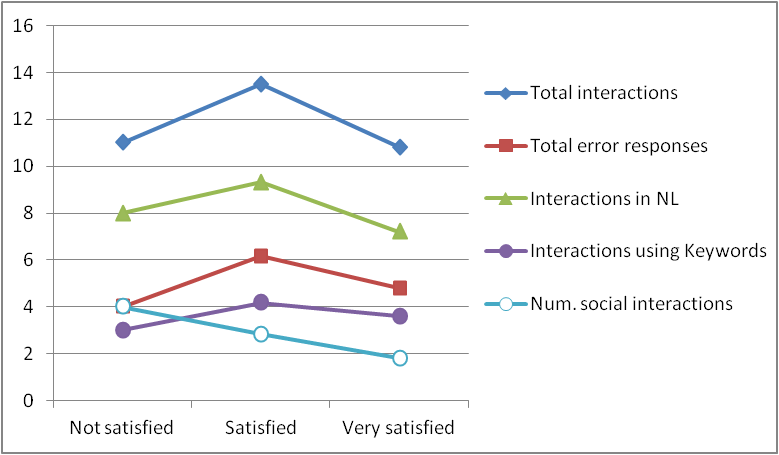
\includegraphics[width=0.8\textwidth]{img/test/exp_satisfaction.png}
  \DeclareGraphicsExtensions.  
  \caption{User interaction metrics sorted by its satisfaction}
  \label{fig:exp_satisfaction}
\end{figure}



